\documentclass[11pt,a4paper]{article}
\usepackage[margin=2.2cm]{geometry}
\usepackage{graphicx,amsmath,amssymb,booktabs,xcolor,hyperref,float,caption}
\captionsetup{font=small,labelfont=bf}
\graphicspath{{figs/}}
\DeclareGraphicsExtensions{.pdf,.png}
\newcommand{\half}{\tfrac12}
\newcommand{\la}{\ell_a}
\newcommand{\kT}{k_BT}
\newcommand{\hyp}{\textbf{\textcolor{orange!80!black}{[hypothesis]}}}
\newcommand{\supp}{\textbf{\textcolor{green!50!black}{[supported]}}}
\newcommand{\out}{\textbf{\textcolor{red!70!black}{[ruled out]}}}
\title{What crowding does to the wall layer\\[2pt]\large Escape, depth, tilt, coherence and exchange against wall density}
\author{Notes for B.~Loewe and T.~N.~Shendruk (prepared with Claude)}
\date{22 October 2026 (revised the same evening: escape rates recounted with a predictive tracker, Sec.~\ref{sec:tracker})}
\begin{document}
\maketitle

\begin{abstract}
We know reasonably well what happens in sparse wall layers. Elongation breaks the tilt coherence; a wall $+\half$ untilts over about 40\,t.u., its
jet turns inward and it leaves. This report is about the crowded side. All results are at $\zeta=0.07$ and come from the 675-run shape sweep
(circles, ellipses and Cassini ovals; $R_{\rm eq}=1$--$2\,\la$; five wall densities $\rho=2k/P\approx0.04$--$0.14$; 3 seeds), plus the existing channels.

\begin{itemize}
\item \textbf{Escape.} Crowding lowers the escape rate of a wall defect by about 18$\times$ in elongated cavities, about 10$\times$ at aspect 1.1--1.3, and only about 2$\times$ in circles. (The first version said about 100$\times$; the old tracker missed fast escapes, most of them in crowded layers; Sec.~\ref{sec:tracker}.) The rate follows the density of the whole layer. A defect's own tilt does not predict it, and neither does its spacing to its neighbours.
\item \textbf{Push model.} The per-defect jet-push model predicts no density dependence, so it cannot explain the drop.
\item \textbf{Elastic pull.} The one-constant elasticity of the layer gives a restoring force on a leaving defect that grows with density. In sparse layers the discreteness of the layer cancels most of the pull of the hole the defect leaves behind. In crowded layers the layer acts as a smooth line of charge (a Gauss-law limit), and the full pull acts. The peak force is close to $\pi^2K\rho/2$. The same elasticity sets the layer depth exactly.
\item \textbf{Barrier in measured configurations.} The barrier computed from measured configurations grows by $\times2.5$ with density. Before today it had only been reported pooled over densities. In crowded layers, the defects that leave already face a lower barrier 40\,t.u.\ before leaving.
\item \textbf{Coherence.} Crowded circles lose tilt coherence through defects that untilt and sit at the wall. Most stay, but they leave 5--10$\times$ more often than the majority. The near-wall flow does not lose coherence.
\item \textbf{Who leaves.} In crowded layers the leavers are squeezed defects (nearer neighbour unusually close). Squeezing alone lowers the elastic climb by as much as the measured escaper deficit. In sparse layers the leavers sit at the tips.
\item \textbf{Kinetics vs steady state.} Crowding blocks exits but not entries, and it restores a stationary layer in elongated cavities. It changes the steady bulk charge per length by only about 35\%. The channels behave in the same way.
\item \textbf{Channels: no topological current.} The mid-line ``current'' of mixed-winding channels was a tracking artefact; an exact topological check gives zero (Sec.~\ref{sec:tracker}).
\item \textbf{Fig.~1(c) of the PRL.} The charge does add up. The ``vacancies'' at large $R$ are defects 4--12 cells from the wall (a diffuse layer) that neither panel counts.
\end{itemize}

Each claim below is tagged \supp, \hyp\ or \out.
\end{abstract}

\tableofcontents
\bigskip

\section{Tracker correction (revised evening of 22 October)}\label{sec:tracker}
\textbf{What went wrong.} Every escape count in the first version linked a defect to its nearest same-sign neighbour in the next frame, within a fixed radius and with no motion prediction:
\begin{itemize}
\item \texttt{shape\_runs.csv} and the per-event data use frames every 10\,t.u.\ and links under 6 cells, which caps the speed at 0.6 cells/t.u.;
\item the exchange counts use 2\,t.u.\ frames and 3.5-cell links.
\end{itemize}
In cavities 4--10\% of bulk defects move more than 3.5 cells per 2\,t.u.\ frame (99th percentile 10--16 cells). Crowded escapers are \emph{fast}: 0.71 cells/t.u.\ on average, against 0.52 for sparse ones. The old chain therefore dropped most crowded escapes and few sparse ones, so the undercount grows with crowding: $\times1$--2 sparse, $\times6$--20 crowded.

\textbf{New tracker.} Each defect's next position is predicted from its last displacement, all defects are matched at once (Hungarian assignment), the gate is 9 cells, and a track may miss up to 2 frames. Results are the same with a 6-cell gate. Escape trajectories are continuous: the largest single-frame step has a median of 3 cells, and 1\% exceed 6.

\textbf{Exact checks.} The charge enclosed by any closed curve can only change by crossings, because pair creation and annihilation are neutral.
\begin{itemize}
\item \textbf{Channels.} The mid-line is such a curve. Its enclosed charge $Q_{\rm up}(t)$ is flat in every run, so the mixed-channel ``topological current'' of 0.03--0.06 per length per 1000\,t.u.\ (channel analyses of 15--16 Oct) is a tracking artefact. The new tracker reproduces $Q_{\rm up}(t)$ (end value $+1.0$ against $+0.9$; rms 2). Details: \texttt{channel/CURRENT\_WITHDRAWN.md}.
\item \textbf{Cavities.} The charge beyond 4 cells is flat in every run.
\end{itemize}

\textbf{Corrected escape probability} (per wall defect per 20\,t.u., predictive tracker; file \texttt{shape\_esc2.csv} in \texttt{crowd\_protect/exchange}). Medians over runs; the old values are in brackets.
\begin{center}\begin{tabular}{lccccc}\toprule
$\rho$ & 0.04 & 0.06 & 0.09 & 0.12 & 0.14\\\midrule
aspect $\geq1.4$ & 0.162 (0.072) & 0.099 (0.056) & 0.038 (0.017) & 0.013 (0.0021) & 0.0088 (0.0007)\\
aspect 1.1--1.3 & 0.029 (0.017) & 0.020 (0.013) & 0.010 (0.004) & 0.0037 (0.0006) & 0.0029 (0.0001)\\
circles & 0.0050 (0.0051) & 0.0030 (0.0025) & 0.0031 (0.0011) & 0.0025 (0.0003) & 0.0022 (0.0002)\\\bottomrule
\end{tabular}\end{center}
\textbf{What survives.}
\begin{itemize}
\item Crowding protects elongated layers ($\times18$).
\item Coherence gates the leak: incoherent layers leak 5--10$\times$ more than coherent ones at every $\rho$, and the step is now sharp at every density.
\item Entries are barely slowed (refill per bulk $+\half$ falls about $2\times$, escapes about $18\times$; 27 Oct recheck).
\item The per-event nulls hold: own tilt, local spacing and depth do not predict escape.
\item Squeezed defects leave in crowded layers.
\end{itemize}
\textbf{What changes.} All the magnitudes; crowding barely protects circles; and near-radial or wrong-sign defects in crowded circles do leave more often than the majority. Figures \ref{fig:alts}, \ref{fig:force} and \ref{fig:exch} use the corrected counts. Validation tests and checking movies for the trackers: \texttt{crowd\_protect/tracker\_validation} (in progress).

\section{Fig.~4 pooled densities; the leak at fixed density}
\textbf{What we did.} Panels (a,b) of PRL Fig.~4 took medians over seeds and $k$ for each family, aspect and size. Each point therefore mixed five
wall densities. We split the data by density.

\textbf{Results.}
\begin{itemize}
\item The loss of tilt coherence $C$ with aspect is nearly the same at every density: $C\approx0.4$--$0.55$ at aspect $\geq1.6$.
\item The leak is not. At aspect 2, sparse walls ($\rho=0.04$) have 45--55\% of their sites empty; crowded walls ($\rho=0.14$) have 3--6\%.
\item Within each density, the vacant fraction tracks $C$ (rank correlation $-0.73$ to $-0.86$). Aspect adds little once $C$ is known.
\item The escape rate steps up by $\times5$--10 when $C$ drops below about 0.85, then levels off. Density sets the level ($\times\sim20$; corrected counts).
\item With the corrected counts the step is sharp at every density. At aspect 1 every density escapes at about $3\times10^{-3}$: crowding only protects once elongation has broken coherence. (The first version saw a gradual rise in crowded walls; that was the tracker.)
\end{itemize}
The current Fig.~4(b) is now the vacant fraction against aspect, one curve per $\rho$. Fig.~\ref{fig:alts} shows six candidate replacements for
the top row; the choice is open.

\begin{figure}[H]\centering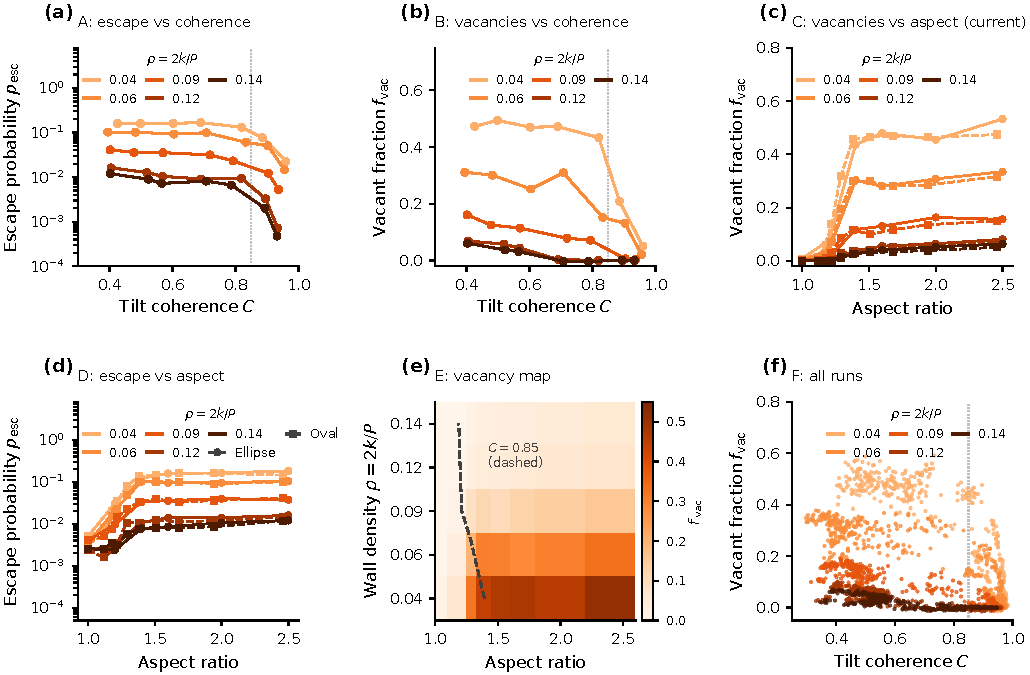
\includegraphics[width=\textwidth]{fig4b_alternatives}
\caption{Candidates for Fig.~4(b). (a) Escape probability against coherence $C$, per $\rho$ (binned medians, log scale). (b) Vacant fraction against $C$.
(c) Vacant fraction against aspect (the current 4b). (d) Escape probability against aspect. (e) Map of the vacant fraction over aspect $\times\,\rho$ with the
$C=0.85$ contour. (f) All runs. In every panel, coherence loss switches the leak on and density sets its size.}\label{fig:alts}\end{figure}

\section{Escape against crowding: run level and per event}
\textbf{Run level, at matched tilt.} Tilt and density are strongly correlated across runs ($r=-0.8$ to $-0.94$). In the tilt bins where both
vary, the escape probability falls by 30--200$\times$ from sparse to crowded walls (corrected counts). At fixed density it changes much less with tilt.

\textbf{Per event} (corrected outcomes from the predictive tracker, \texttt{events2.npz}). We followed every resident wall $+\half$ in the sweep: $5.4\times10^6$ starting positions, $1.2\times10^5$ escapes within 20\,t.u.\ and $7.9\times10^4$ lagged escapes. We compared defects
within the same run, using Mantel--Haenszel odds ratios: each run is split at its own median, so run-level differences cancel.
\begin{itemize}
\item \textbf{Escape within 20\,t.u.} The defect's own tilt and depth look like strong predictors (odds ratios 0.40 and 4.8). This is the known run-up: escapers untilt and move inward before leaving.
\item \textbf{Lagged escape.} The outcome is: still in the wall at $+40$\,t.u., deeper than 6 cells at $+60$\,t.u. Tilt has no effect (1.03) and nor does depth (1.01). Local spacing has a weak effect (0.96; $\times1.27$ between the top and bottom spacing quartiles in sparse runs, $\times0.52$--0.57 in crowded ones).
\item \textbf{Lagged escape by density.} Per 1000 starts it is 44.5, 42.9, 20.3, 6.6 and 4.9 for $\rho=0.04$--0.14 (first version: 23, 24, 10.5, 1.3 and 0.36).
\end{itemize}
\supp\ Escape is set by the density of the whole layer, not by a defect's own tilt or its local spacing. The earlier line ``tilt sets rates,
crowding sets the steady state'' is withdrawn.

\textbf{The PRL exit-vs-vacancy numbers.} The PRL quotes 0.068 per wall defect per 20\,t.u.\ for a full layer and 0.028 with five vacancies. These come
from 49 runs that all have $k=6$, so the density is fixed and the vacancies are frame-to-frame fluctuations. With each run's mean removed, the
numbers become 0.065 and 0.021, so they hold. The shape sweep at fixed $\rho$ shows a weaker version of the trend ($-20$--30\%, then flat). The two
effects are separate. The density imposed by the winding changes escape about 9--18-fold (corrected); the vacancies present at a given moment change it by $\times1.3$--3.

\section{Why crowded layers do not leak: tests}
\subsection{Jet-push model \out}
The existing model has push $P=0.40\cos\tau\,g(d)$, where $g$ is the fraction of the inward jet that the wall lets through, with a logistic exit
probability fitted on the $k=6$ runs. Applied to every resident defect, it predicts the same exit probability at every density (ratios 0.98--1.06),
while the measured one falls $\times2.4$ (circles) to $\times17$ (elongated) with the corrected counts. Crowded defects sit shallower, so less jet gets through, but they are also less tilted (larger
$\cos\tau$). The two effects cancel.

\subsection{Depth memory}
Fluctuations in a resident's depth decorrelate in 2--6\,t.u., and its tilt in 14--18\,t.u. The 40\,t.u.\ lagged test therefore could not have
seen a depth effect. Depth averaged over 20\,t.u.\ is a weak lagged predictor (odds ratio 1.2--1.6).

\subsection{Near-wall flow \out\ (as the main cause)}
Near-wall speed and shear are similar at every density; the shear is up to 30\% higher when crowded. The rms inward flow 2--6 cells from the wall is
20--27\% lower in crowded layers, and its peak moves from about 6 cells to about 2.5. That is not enough for the $\times18$ suppression. Caveat: the flow
fields are saved every 100\,t.u., and we did not check whether they are time averages.

\subsection{Elastic pull on a leaving defect \supp}
\textbf{What we did.} We used the one-constant Frank energy with $K=44\,\kT$ and rigid cores of radius 1.5, in a circle with perimeter $P=200$: a
ring of $N$ wall $+\half$ at the depth-law radius plus a central $+1$. One wall defect is dragged radially inward with all others fixed. Two
versions: (i) the relaxed field on a grid with core orientations held or free; (ii) the analytic point-charge energy with wall images. They agree
within a few $\kT$.

\textbf{Gauss split.} We write the other $N-1$ wall charges as three pieces:
\begin{itemize}
\item a smeared uniform ring of all $N$ charges;
\item a hole of charge $-\half$ at the dragged defect's starting site;
\item the remainder, the corrugation from discreteness.
\end{itemize}
By the 2D shell theorem the smeared ring exerts no force inside it, which is true to $\leq0.3\,\kT$. What resists leaving is the hole (with its image)
plus the corrugation.

\textbf{Results} (Fig.~\ref{fig:drag}, Fig.~\ref{fig:force}).
\begin{itemize}
\item The cost of a 6-cell drag with the tilt held at $60^\circ$ is 64, 91, 117, 144 and 149\,$\kT$ for $\rho=0.04$--0.14.
\item Holding the tilt (0--$90^\circ$) or letting it rotate changes the cost by at most about $8\,\kT$ (mostly $\leq5$), consistent with the per-event tilt null.
\item The hole term is 147--182\,$\kT$ at every density. The corrugation term is $-85$, $-61$, $-31$, $-8$ and $+5\,\kT$.
\end{itemize}
In a sparse layer (spacing about 30 cells) a defect 6 cells out never sees a clean hole in a smooth line, and the lumpiness cancels most of the
pull. In a crowded layer (about 7 cells) the layer is already smooth at that distance, and the full hole pull acts.

\textbf{Force against $N$.}
\begin{itemize}
\item The zero of the radial force on the whole ring reproduces the depth law exactly. The measured depths (minus the usual 0.61-cell offset) match in crowded layers; sparse layers sit about 0.5 cells shallower.
\item For a single leaving defect, crowded layers have a force peak at 1.5--2 cells. The peak is close to the line-charge value $\pi^2K\rho/2$: 32\,$\kT$/cell at $\rho=0.14$.
\item Sparse layers have no peak; the force rises slowly towards the Coulomb pull of the hole (15\,$\kT$/cell at $\rho=0.04$).
\item Beyond about 6 cells every density converges to the Coulomb pull of the hole and its image. That is the Gauss limit in the bulk.
\item The measured escape falls roughly exponentially with the peak force: $\times18$ from 15 to 32\,$\kT$/cell in elongated cavities (corrected counts; the first version said $\times100$), and only $\times2.3$ in circles. This is a correlation through $\rho$ only.
\end{itemize}

\textbf{Barrier in measured configurations.} The escape analysis already computed the elastic climb from measured configurations (anisotropic $K$;
6-cell cost $E_6$, initial force $F_0$), but pooled over densities. Split by $\rho$, the residents give $E_6=41$, 64, 86, 101 and 102\,$\kT$, and
$F_0=-5.6$ to $-15.1\,\kT$/cell. That is the same $\times2.5$ as the clean calculation.

\textbf{Who leaves (pairing at fixed $\rho$) \supp.} We paired escapers with residents from the same run, the same frame and the same region:
\begin{itemize}
\item Sparse layers ($\rho\leq0.06$): escapers face the same climb at every lead time ($\pm$1--3\,$\kT$). Elasticity does not pick who leaves.
\item $\rho=0.12/0.14$: escapers face a lower climb already 40\,t.u.\ before departure ($-8\pm4$, $-14\pm4\,\kT$), and $-14/-27\,\kT$ at 20\,t.u.
\end{itemize}
In crowded layers the defects that leave are the ones that happen to face a weaker pull. (Caveat: the escapers in this energetics sample were identified with the old tracker, which kept mostly the slower escapes in crowded layers.)

\textbf{What makes the pull weaker: squeezing \supp} (\texttt{crowd\_protect/who\_leaves.txt}, \texttt{squeeze\_barrier.txt}). These are lagged escapes ($\geq40$\,t.u.\ ahead), with within-run percentiles.
\begin{itemize}
\item In crowded elongated layers the escapers are squeezed. Their nearer neighbour is at the 39th percentile, and escape is $\times2.3$ more likely in the most-squeezed quarter. Asymmetric gaps and flank positions matter slightly.
\item In sparse layers gaps are irrelevant and the tips dominate ($\times1.4$).
\item \textbf{Analytic check.} Shifting a defect 0.3--0.4 of a spacing towards a neighbour lowers its 6-cell climb by 15--28\,$\kT$ ($N=24$--28), which matches the escaper deficit. The squeezed state itself costs 20--37\,$\kT$, so it is rare and must be made by the activity.
\end{itemize}

\begin{figure}[H]\centering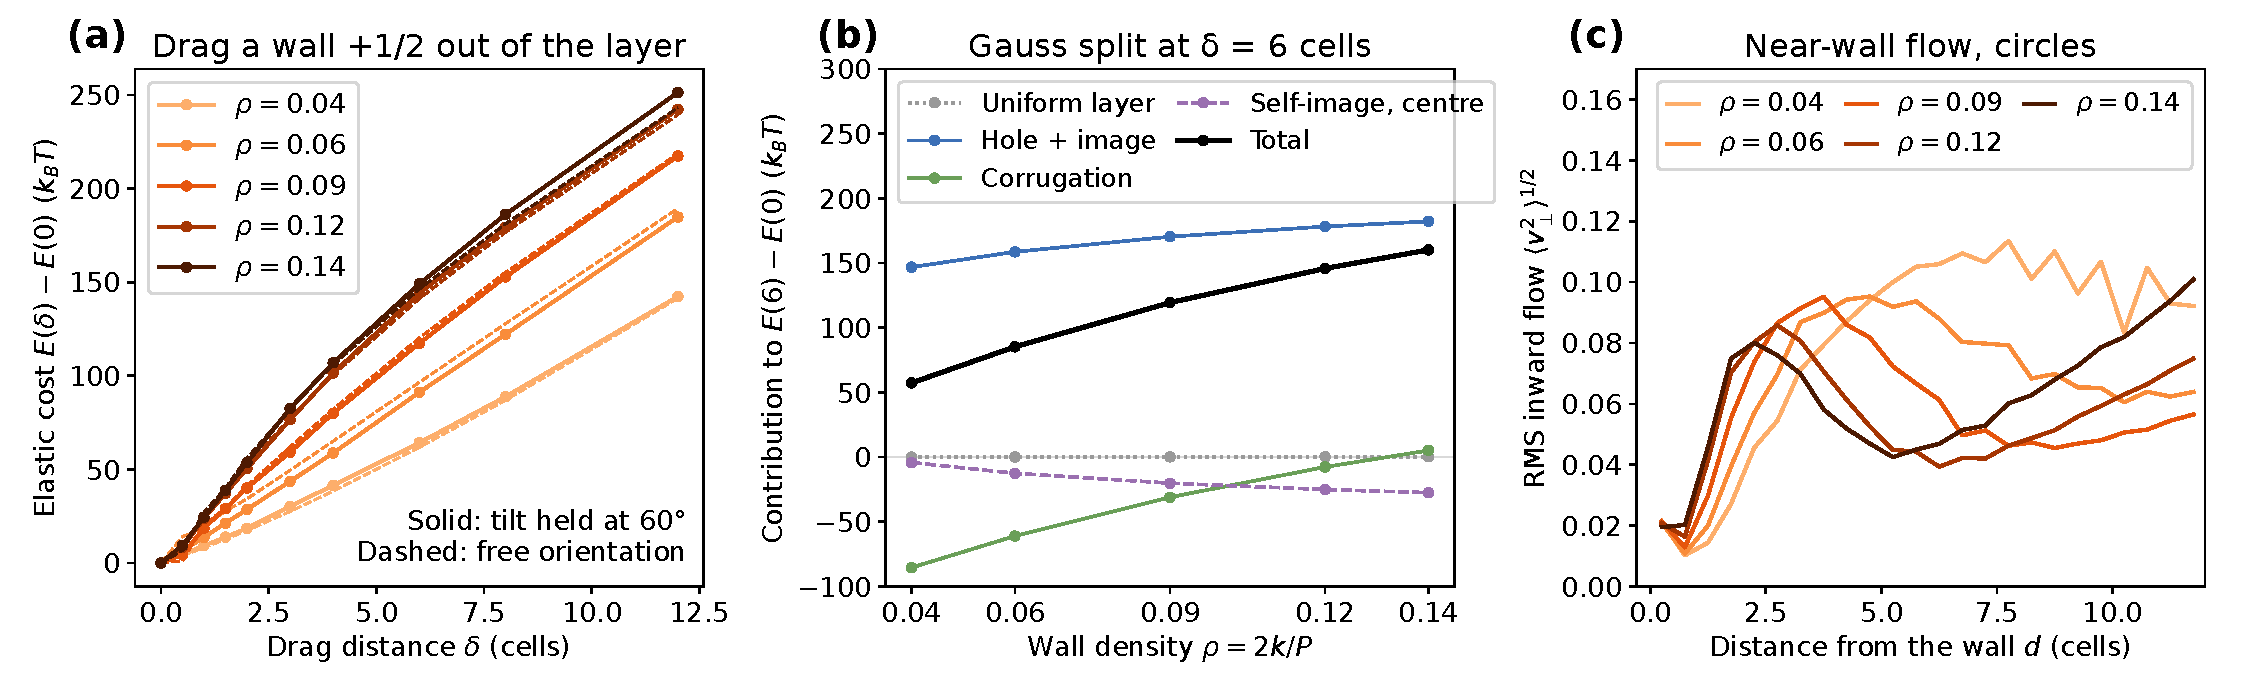
\includegraphics[width=\textwidth]{fig_crowd_protect}
\caption{(a) Elastic cost of dragging one wall $+\half$ inward (one constant, $K=44$; solid: tilt held at $60^\circ$, dashed: free). (b) Gauss split of
the cost at 6 cells: uniform layer (zero, shell theorem), hole $+$ image, corrugation (discreteness), self-image $+$ central charge. (c) RMS inward flow
against wall distance, circles.}\label{fig:drag}\end{figure}
\begin{figure}[H]\centering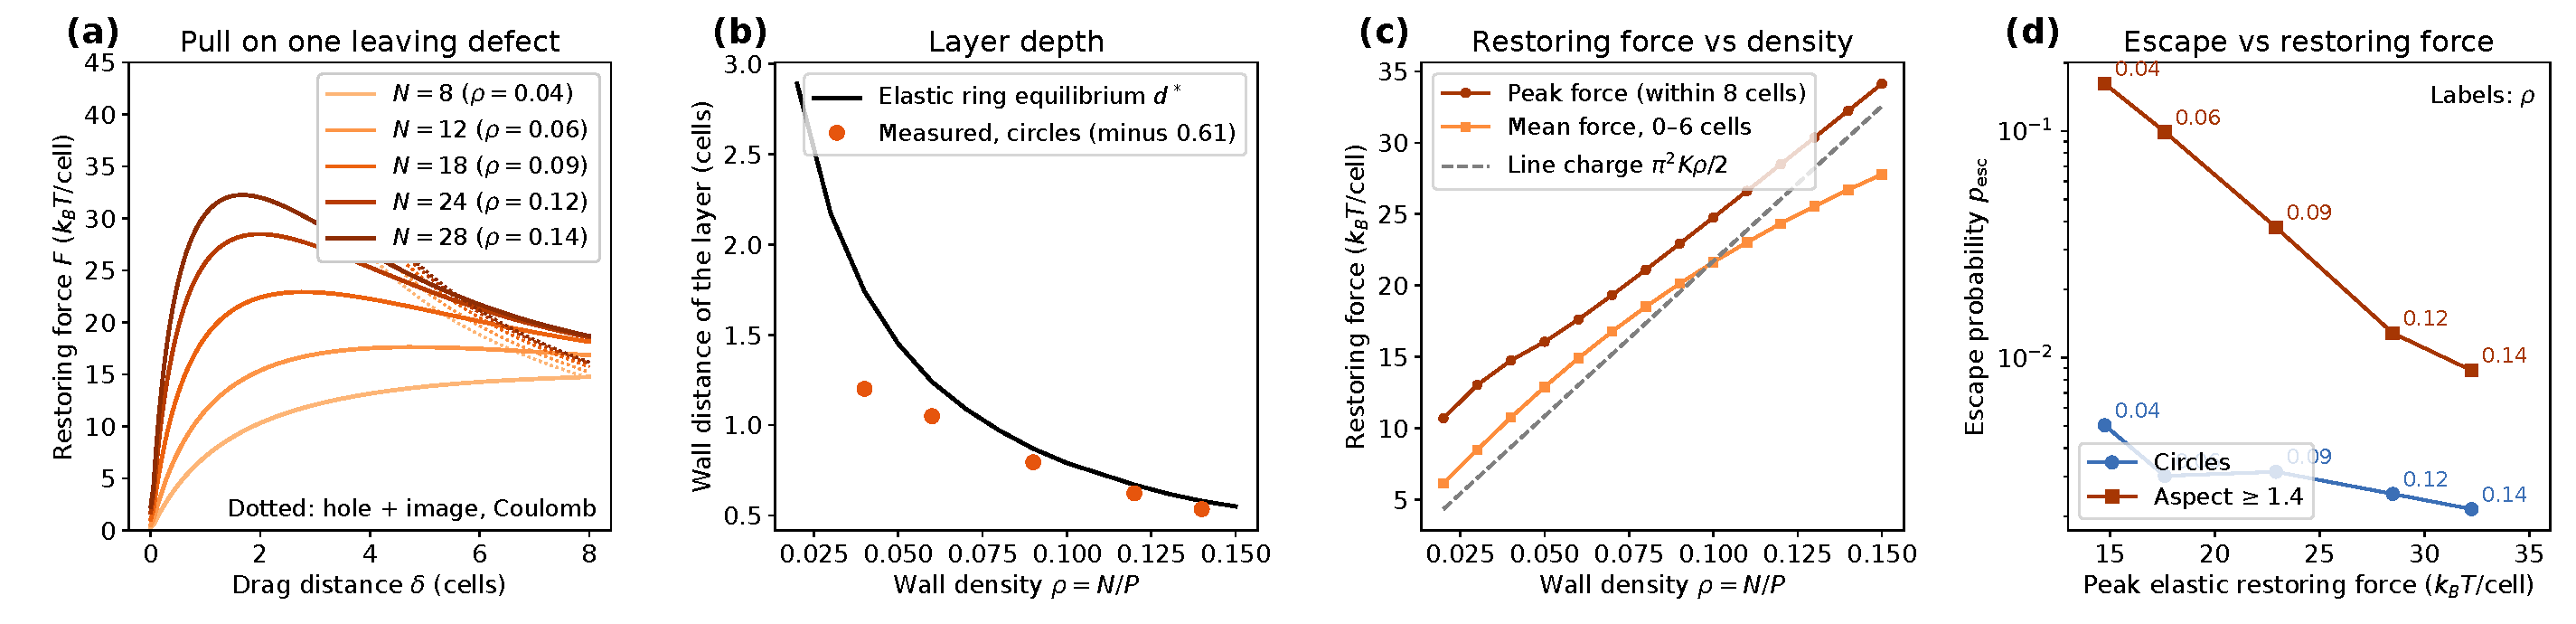
\includegraphics[width=\textwidth]{fig_force_vs_N}
\caption{(a) Restoring force on one leaving defect for five $N$ (dotted: Coulomb pull of hole $+$ image). (b) Equilibrium wall distance of the ring
(force zero) and measured depths. (c) Peak and mean restoring force against $\rho$ with $\pi^2K\rho/2$. (d) Measured escape probability against the
peak force.}\label{fig:force}\end{figure}

\section{Coherence loss in crowded layers}
\textbf{Your hypothesis:} crowded defects sit closer to the wall, where the flow is weaker, so MPCD noise wins.
\begin{itemize}
\item \textbf{Flow.} The flow along the wall 1--3 cells out is \emph{more} coherent when crowded: $|\langle v_t\rangle|/\langle|v_t|\rangle$ goes from 0.83 to 0.95. Circulation is unchanged, and the shear at the core depth is similar or larger. Only the flow speed at the core is lower (by about 35\%). The flow is not the cause.
\item \textbf{Where the wrong-sign defects sit.} In crowded circles they mostly sit just past radial: a peak near $-10^\circ$ with a shoulder to $-90^\circ$, not at the mirror tilt (Fig.~\ref{fig:coh}b). Near-radial ($|\tau|<20^\circ$) plus wrong-sign defects grow from about 0\% to 9\% and 6\%.
\item \textbf{What they are doing.} They sit at the same depth as the majority or slightly shallower (1.04 vs 1.16 cells). With the corrected counts they leave more often than the majority: lagged escape 8.5 (wrong sign) and 4.4--6.6 (near-radial) against 0.8--1.0 per 1000, so partly failed or slow run-ups. Most, however, stay. (The first version said they essentially never leave.) In sparse circles the rare near-radial and wrong defects are deep (about 3.4 cells) and mostly leaving: run-ups in progress.
\end{itemize}
\supp\ Crowded layers lose coherence through defects that untilt and stay at the wall: your ``untilted defects pushed against the wall''.
Caveat: $C$ is measured from the outward normal, so an untilted defect lowers $C$ only when it crosses past radial.

\textbf{Kinks.} In circles the wrong-sign fraction rises from 0.3\% to 9.6\%, the rate of wrong-sign episodes from 1.2 to 7.9 per defect per 1000\,t.u.,
and their lifetime from 3.7 to 10.8\,t.u. Misread orientations stay at about 1\%. Wrong-sign defects cluster (about 1.4 clusters per ring at
$\rho=0.14$; independent flips would give about twice as many sign changes).

The elastic cost of a wrong-tilt defect that slides to its own lock site is about 17--21\,$\kT$ at $\tau=55^\circ$, roughly flat in $N$. It depends
strongly on the tilt (5, 18 and 28\,$\kT$ at 30, 55 and 65$^\circ$). \out\ My earlier statement that kinks get cheaper because the lock softens.
\hyp\ Kinks get cheaper because crowded layers tilt less, which ties them to depth.

\textbf{Depth and tilt per defect} (\texttt{crowd\_protect/depth\_tilt.txt}; 20\,t.u.\ window means, within runs). In crowded layers deeper defects are more tilted: $+13^\circ$/cell in circles at $\rho=0.12$--0.14 (none at 0.04), and $+21$--$24^\circ$/cell in elongated cavities. Across densities, the circles' layer depth falls 0.66 cells while its tilt falls $12^\circ$ (about $18^\circ$/cell), the same order. This supports a depth-to-tilt chain in crowded layers, but the correlation is weak (rank 0.10--0.14) and the direction of cause is open. Kink statistics use wall defects, which are slow, so the old linking is adequate there.

\begin{figure}[H]\centering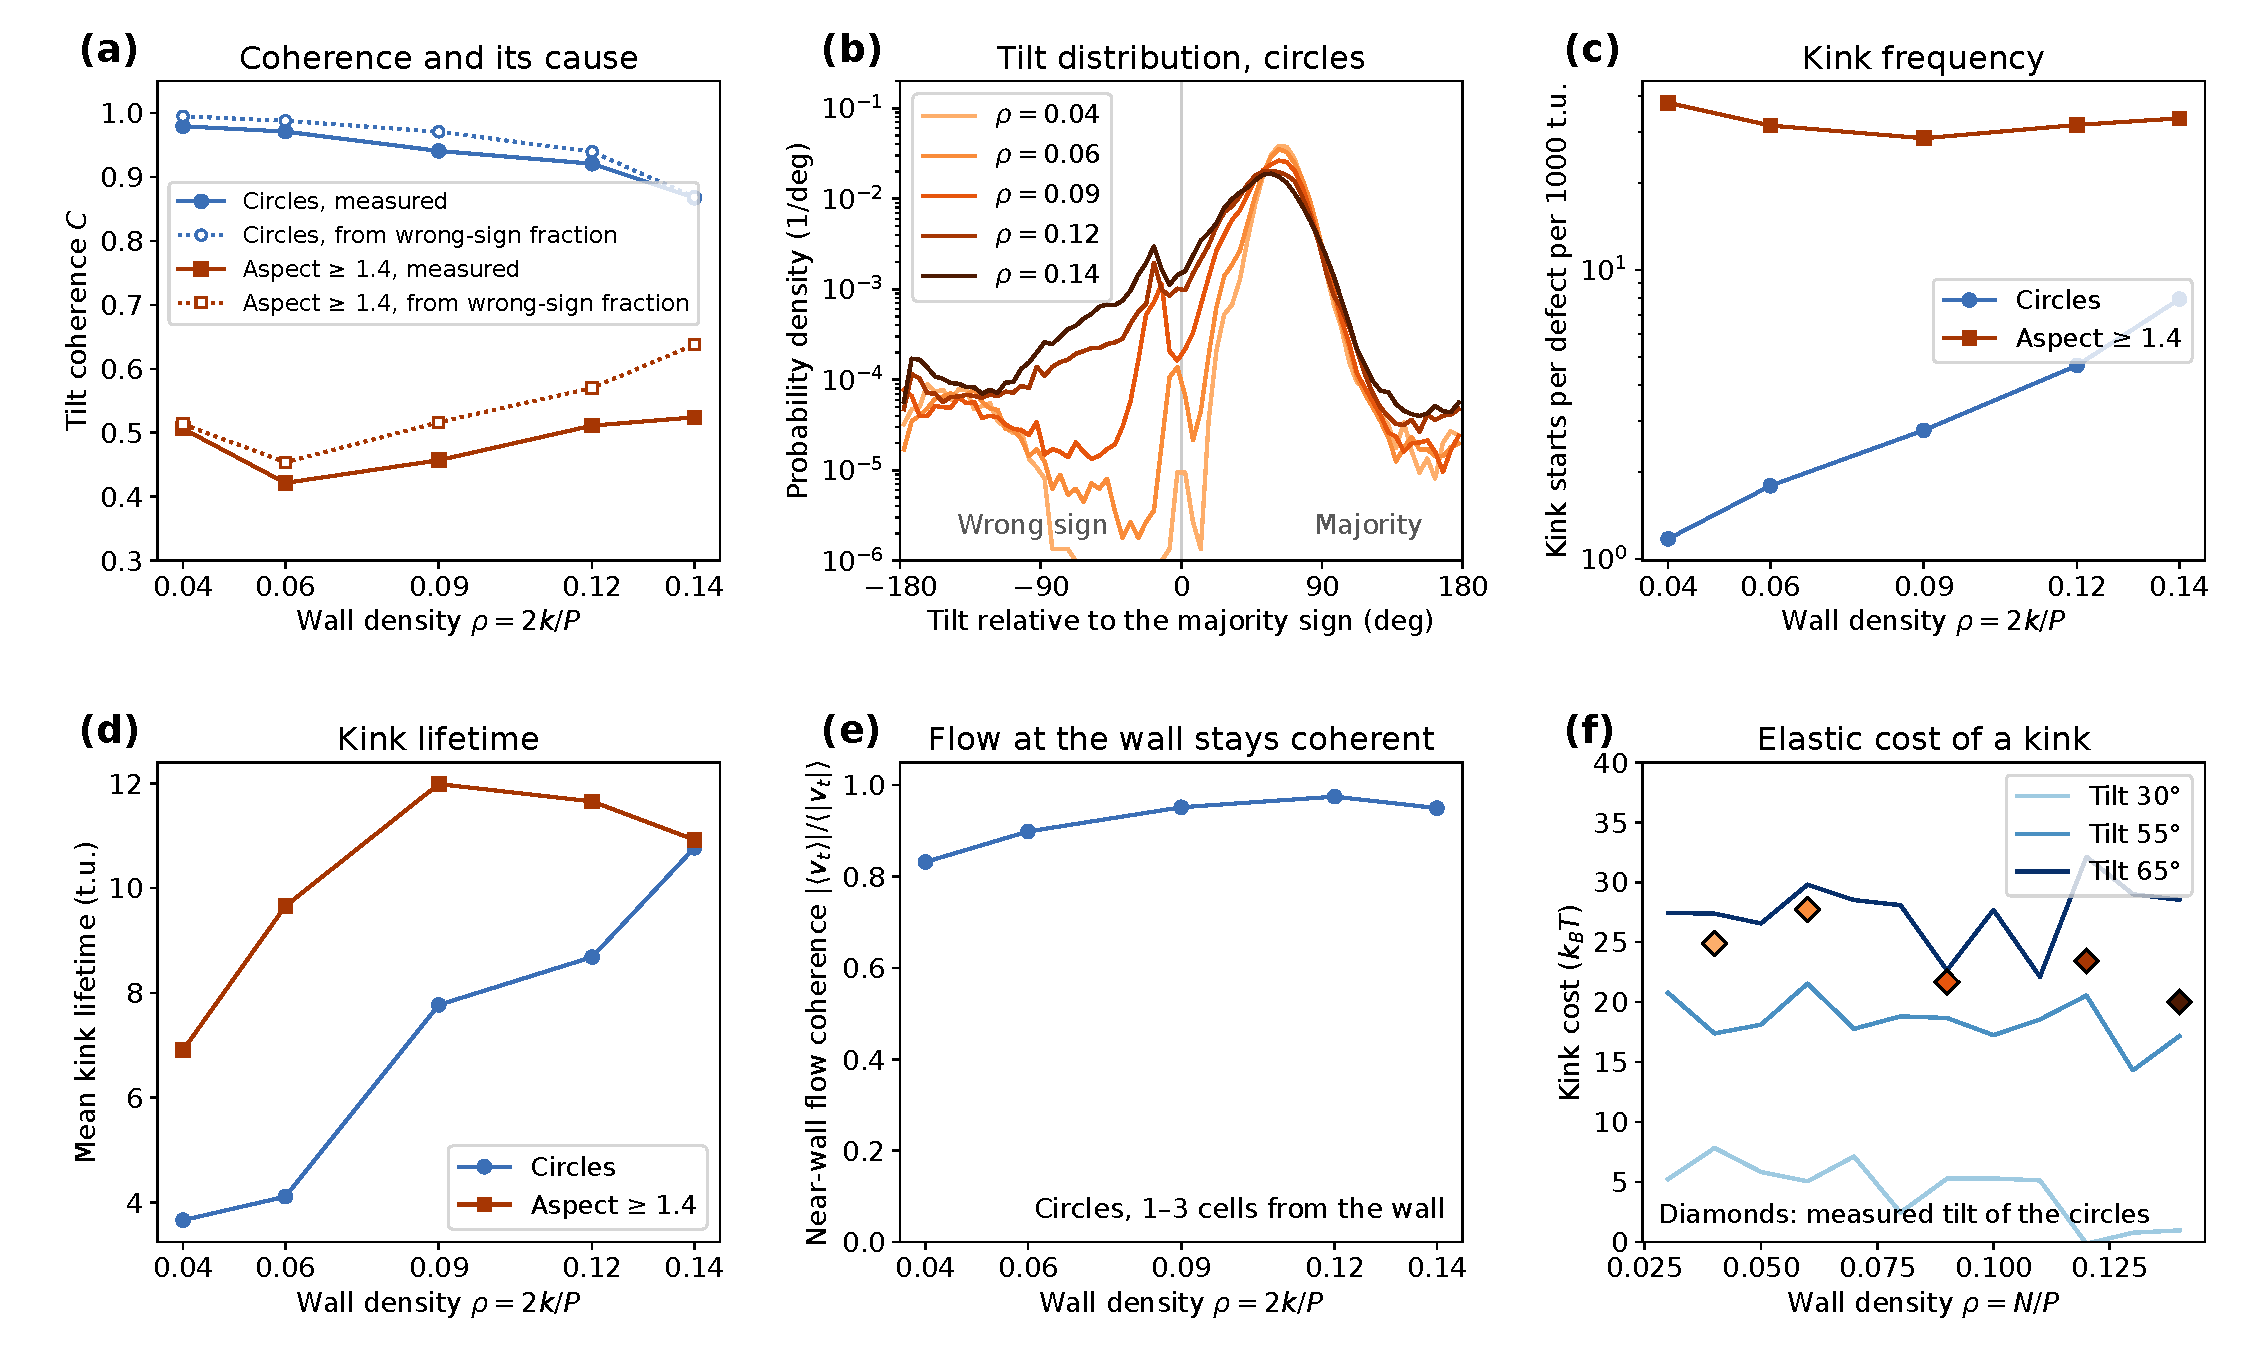
\includegraphics[width=\textwidth]{fig_coherence}
\caption{(a) Coherence $C$, measured and predicted from the wrong-sign fraction and the majority tilt alone. (b) Tilt histograms (circles) relative
to the majority sign. (c) Kink start rate and (d) lifetime. (e) Near-wall flow coherence (circles). (f) Elastic cost of a one-defect kink against $N$
for three tilts; diamonds at the measured circle tilts.}\label{fig:coh}\end{figure}

\section{Kinetics against steady state; channels; stationarity}
\textbf{Bulk charge.} In the channels the bulk charge per length barely moves with crowding. From $m=3$ to $m=12$--24 it goes from about 0.023 to 0.014,
while the released fraction falls from 73\% to 6\%. The cavities behave the same way:
\begin{itemize}
\item circles: flat;
\item elongated: $-35\%$, while the escape rate per defect falls $\times18$ (corrected).
\end{itemize}

\textbf{Tracked exchange.} A clean escape is $\geq20$\,t.u.\ in the wall, then into the bulk, with no return for 20\,t.u. A clean entry is the mirror
image (Fig.~\ref{fig:exch}a). With the predictive tracker, in elongated cavities the escape hazard per wall defect is 11.5, 6.3, 2.05, 0.69 and 0.44 per 1000\,t.u.\ (first version 9.7 \dots\ 0.17); the entry
hazard per bulk $+\half$ is 2.9--4.8, not slowed. Circles have few clean escapes at any density (0.06--0.14). The channels behave like the elongated cavities: escape 22, 4.5, 1.0 and 0.48 at $m=3$, 6, 9 and 12, with entry 1.4--3.1.

\supp\ Crowding is a one-way valve: it blocks exits and barely slows entries (refill per bulk $+\half$ per 20\,t.u.\ falls from 0.09--0.12 to 0.055 in elongated cavities, validated tracker; the old 10\,t.u.\ chain overestimated refill in circles 5--8$\times$).

\textbf{Full charge budget of the wall band, both signs} (\texttt{crowd\_protect/budget}). The budget closes: the residual is 0.001--0.017 against gross fluxes of 0.05--0.6 per length per 1000\,t.u.
\begin{itemize}
\item Crowding cuts gross exchange by 4--7$\times$; pair creation inside the band falls 5--7$\times$.
\item The net $+\half$ flow reverses. Sparse walls are a net source, refilled by pair creation at the wall. Crowded walls are a net sink, emptied by annihilation with incoming $-\half$. Channels flip between $m=9$ and 12.
\item Rechecked with the validated tracker (27 Oct, \texttt{wall\_budget2}). Unpaired births and deaths are 3--5$\times$ smaller (0.002--0.009), and closure against the exact count holds to 1.4 charges. The sign flip survives: sparse elongated walls are a net source ($-0.014$ to $-0.017$), crowded walls a small net sink ($+0.002$ to $+0.003$).
\end{itemize}

\textbf{Stationarity (wall Fourier).} This is the static fraction of the wall density at the lattice mode $2k-2$ (1 = pinned lattice).
\begin{itemize}
\item Circles and aspect $\leq1.3$: 0.93--0.99 at every $\rho$.
\item Aspect 1.35--1.7: 0.27, 0.38, 0.65, 0.75 and 0.77.
\item Aspect 1.9--2.5: 0.04, 0.13, 0.40, 0.50 and 0.51.
\end{itemize}
Sparse elongated layers are the diffuse ones; crowding brings them back to roughly half-pinned.

\textbf{Channel crossover} (Fig.~\ref{fig:cross}; $L=192$, $W=40$, $m=3$--12, validated tracker). The clean escape hazard is 24, 4.6, 3.3, 1.6, 1.07, 0.90, 0.62 and 0.52 per 1000\,t.u.\ for $m=3$, 6, 7, 8, 9, 10, 11 and 12 ($\rho=0.031$--0.125).
\begin{itemize}
\item It falls fast up to $\rho\approx0.08$--0.09 ($\times15$; the largest step is $m=7\to8$), then gently ($\times3$ from $m=8$ to 12).
\item The wall occupancy $N_{\rm wall}/2m$ climbs from 0.28 to 0.79 by $m=9$ and saturates at about 0.84. The layer closes where the push-equals-pull estimate puts the crossover.
\item Entries are flat; the bulk charge per length falls by 25\%; the mid-line current is zero at every $m$.
\item At equal $\rho$, channel escape nearly coincides with elongated cavities. Circles sit 10--30$\times$ lower.
\end{itemize}

\begin{figure}[H]\centering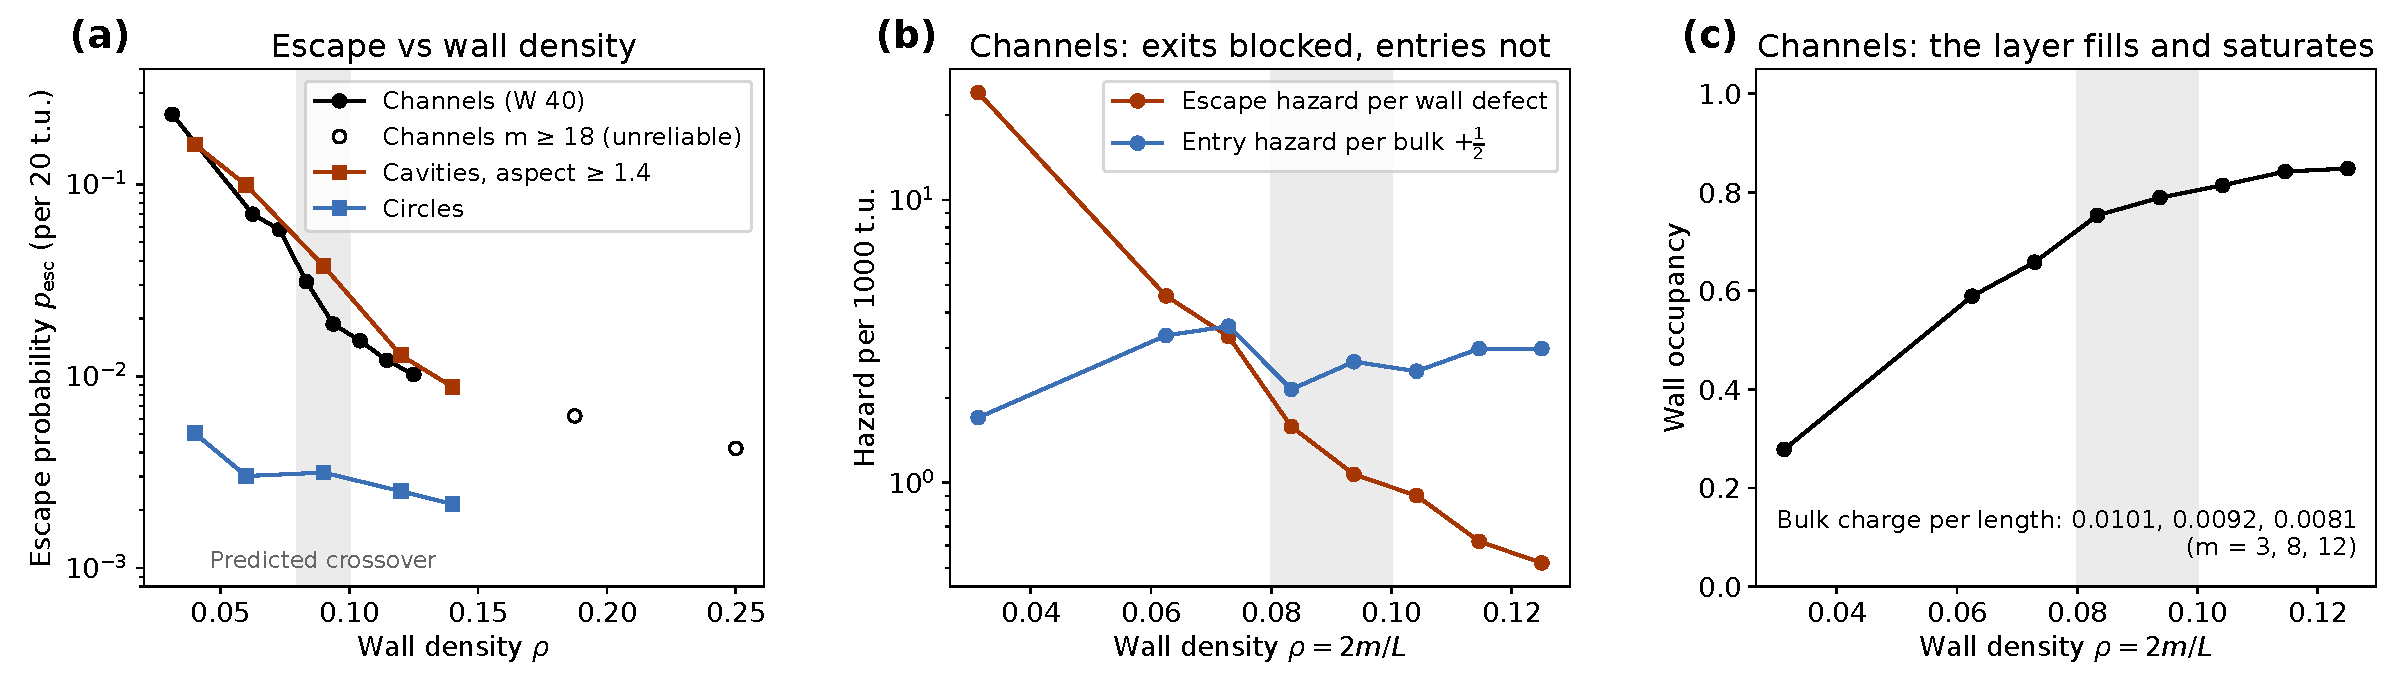
\includegraphics[width=\textwidth]{fig_crossover}
\caption{Channel crossover. (a) Escape probability against wall density: channels ($W=40$), elongated cavities and circles (corrected counts). (b) Clean escape and entry hazards in channels. (c) Wall occupancy in channels. Shaded: predicted crossover.}\label{fig:cross}\end{figure}

\textbf{Drive $\times$ barrier} (\texttt{crowd\_protect/drive\_barrier}; Fig.~\ref{fig:db}). We measured how deep a resident wall $+\half$ gets within 20\,t.u.\ ($S(x)$ = fraction reaching depth $x$).
\begin{itemize}
\item \textbf{The drive (supported).} At every density coherent layers make smaller excursions than incoherent ones.
\item \textbf{The barrier location (supported).} Crowding acts in the first 1.5--2 cells beyond the resident depth, where the crowded-layer pull peaks.
\item \textbf{Near-wall law (supported).} Over the first 2.5 cells, $S\propto e^{-U/T}$, with $U$ the elastic cost of moving out (relaxed-neighbour drag). $T$ is independent of density: $17$--$21\,\kT$ in incoherent elongated layers and $8$--$12\,\kT$ in coherent ones. Measured-configuration energies give the same result: $T=12$--$19\,\kT$ with no trend while the 2-cell cost rises $3.9\times$.
\item \textbf{The deep tail} is kinetic (fast escapers running within the window), so a single $T$ over the full depth fails.
\item \textbf{Circles} are the exception: their $T$ rises $\times2.6$ with density.
\item \textbf{Not supported:} a weaker near-wall drive. The rms inward flow 1--3 cells from the wall rises with density.
\end{itemize}

\begin{figure}[H]\centering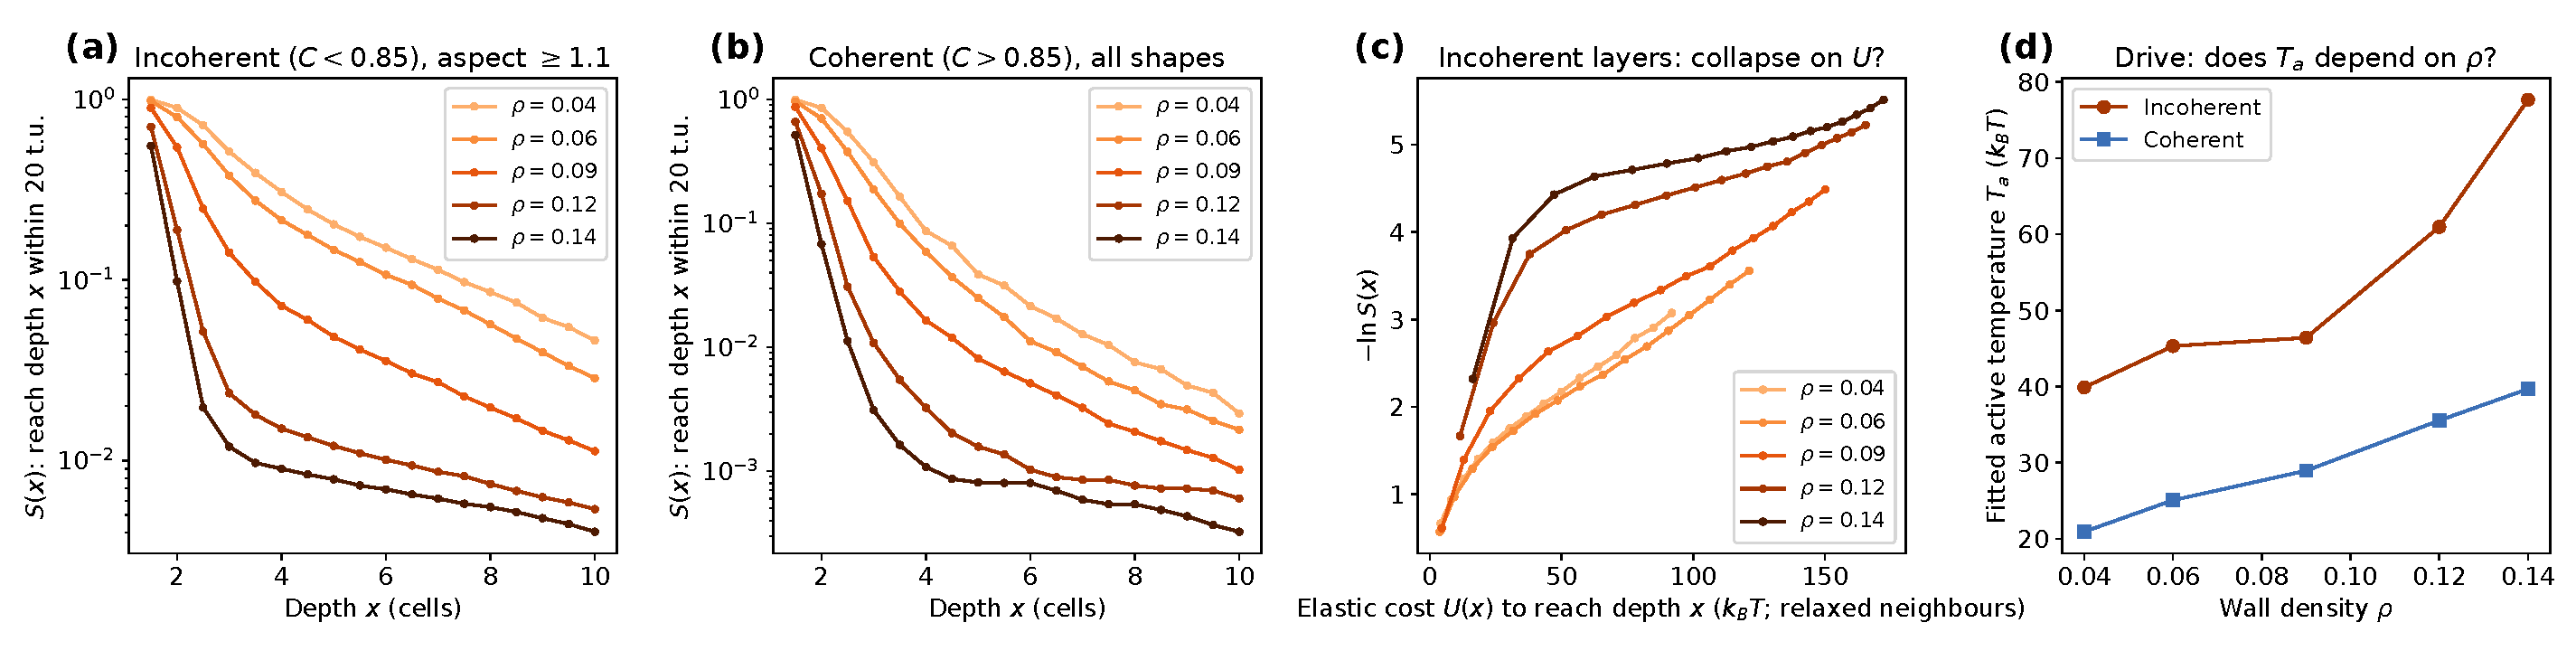
\includegraphics[width=\textwidth]{fig_drive_barrier_relaxed}
\caption{Drive $\times$ barrier. (a,b) Probability $S(x)$ that a resident wall $+\half$ reaches depth $x$ within 20\,t.u., incoherent and coherent layers, per density. (c) $-\ln S$ against the relaxed-neighbour elastic cost (full depth; the near-wall part is linear with a density-independent slope, the deep tail is kinetic). (d) Fitted $T$ over the full depth (the near-wall fit is density-independent; see text).}\label{fig:db}\end{figure}

\begin{figure}[H]\centering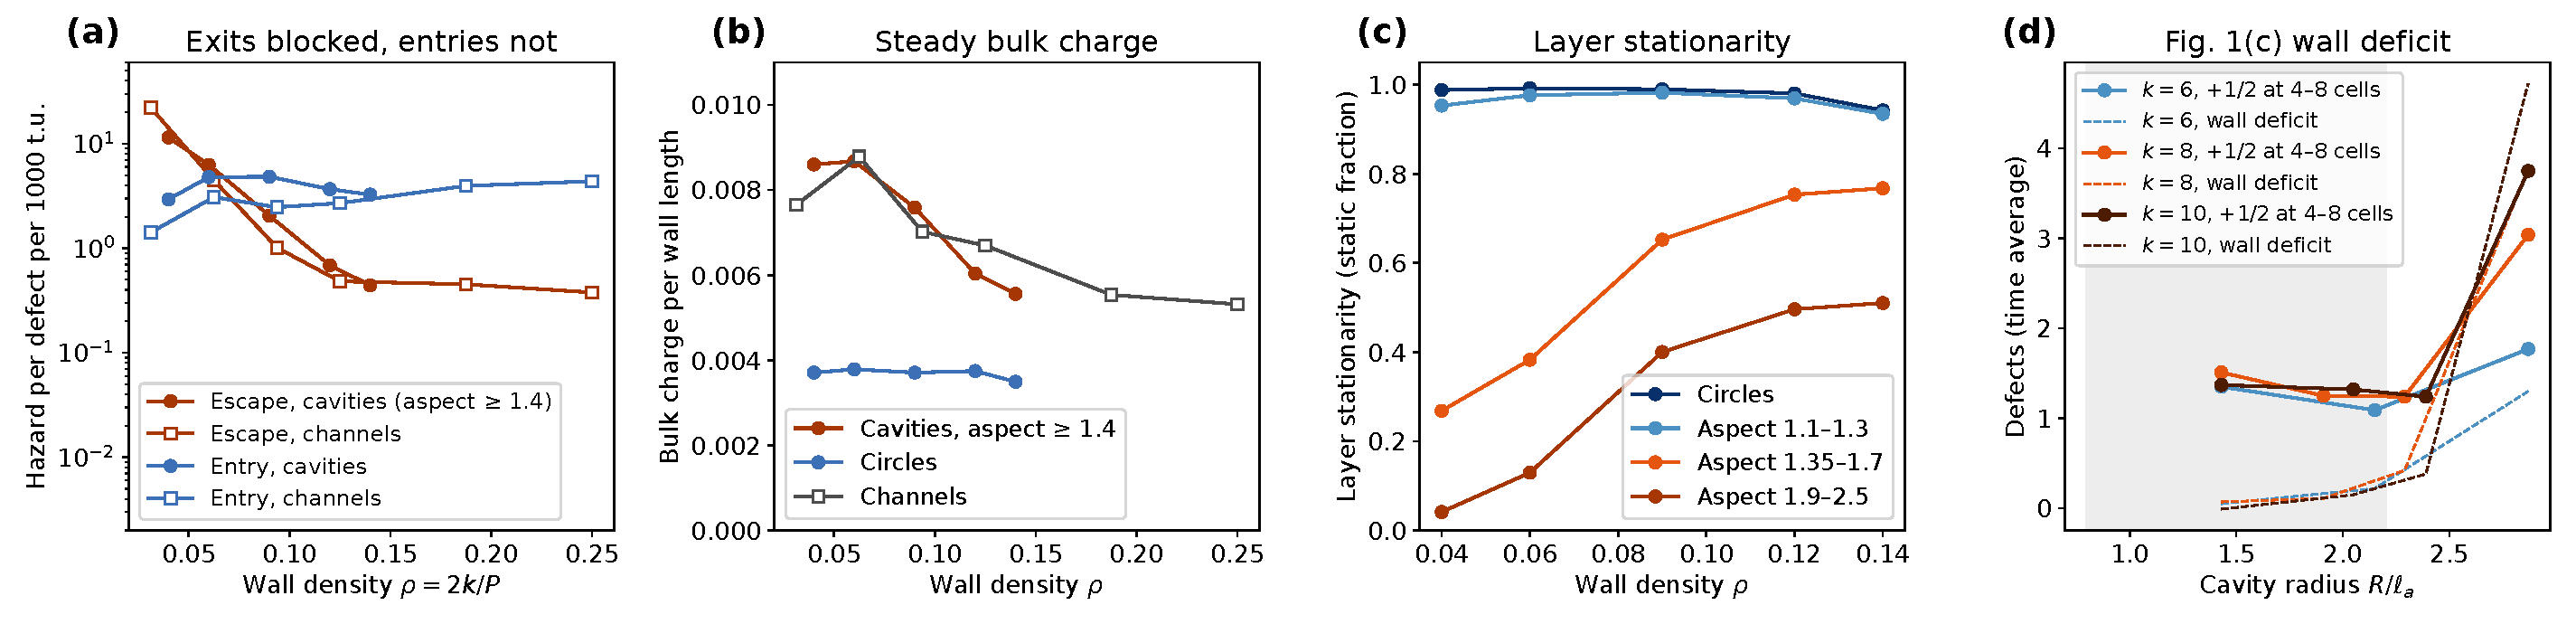
\includegraphics[width=\textwidth]{fig_exchange}
\caption{(a) Clean escape and entry hazards, elongated cavities and channels. (b) Steady bulk charge per wall length. (c) Layer stationarity by aspect.
(d) PRL Fig.~1(c) accounting in large circles: $+\half$ 4--8 cells from the wall against the wall deficit (the rest of the deficit sits 8--12 cells out; see the Fig.~1(c) alternatives, panel D).}\label{fig:exch}\end{figure}

\section{PRL Fig.~1(c): the charge does add up}
\begin{itemize}
\item \textbf{Why the x-values differ between the panels.} The top panel drops any $(k,R)$ that has a knee of $Q(r)$ in fewer than 5 of 10 seeds. That is exactly the large-$R$ points where the wall deficit appears ($k\geq6$ at $R\approx2.6$--$2.9\,\la$ have no knee). The bottom panel's y-range cuts off the smallest-$R$ points, where the wall holds extra defects.
\item \textbf{The two panels count different regions.} The bottom panel counts the wall as $d<4$ cells. The top panel's $Q_{\rm knee}$ is the charge inside the knee radius. Counting charge in bands, the total is exactly $k$ in every run, and the charge outside 4 cells is exactly $1+{}$(deficit)/2.
\item \textbf{Where the deficit sits.} The missing wall defects sit 4--12 cells from the wall, in a diffuse layer, not in the centre. For $k=6$ at $2.87\,\la$ about a third of the missing charge is at 4--8 cells and the rest at 8--12. For $k=10$ at $2.87\,\la$ the wall deficit is 4.7: about half the missing charge is at 4--8 cells and half beyond 8 (correction: an earlier version said all of it sits at 4--8). $Q_{\rm knee}$ stays at 1 where a knee exists, because the plateau sits inside the diffuse layer.
\item \textbf{Why larger $k$ loses more.} These are not crowded layers: beyond the window, $\rho\leq0.06$ for every $k$. Normalised by the number of sites (10-seed medians), $k=6$--8 lose 13--14\% at $2.87\,\la$ and collapse; only $k=10$ is higher (30\%). This is a different phenomenon from today's escape (layer thickening outside the window). Why higher $k$ thickens more is open.
\end{itemize}
Possible fix: plot $k-N_{\rm wall}/2$ for the same 4-cell band in both panels, or count the 4--8 band explicitly and say so in the caption.

\section{Synthesis}
\begin{itemize}
\item \textbf{Sparse walls.} Geometry sets the active flow, and the flow decides tilt, coherence and escape. The layer's own elasticity is weak because its charges are too lumpy to act together. Escapers are not selected elastically.
\item \textbf{Crowded walls.} The layer acts as a smooth line of charge. Its elasticity sets the depth (force zero), the barrier (peak about $\pi^2K\rho/2$) and, through depth, smaller tilt and cheaper kinks. Exits are reduced about 18$\times$ (elongated) and entries are not, and the leavers are squeezed defects with a locally lower barrier.
\item \textbf{Steady state.} The bulk charge per length stays mostly geometric: circles flat; elongated cavities and channels $-35$--40\%. Crowding mainly changes the kinetics.
\item \textbf{Your synthesis, refined.} Topology (the elasticity of the wall charges) overtakes geometry in how fast charge is exchanged, but only modestly in where it ends up.
\item \textbf{Crossover estimate} \supp\ (channels, 27 Oct: escape falls fast and the wall occupancy saturates at $\rho\approx0.08$--0.09). The peak pull equals the active push when $\rho_c=2F_a/(\pi^2K)$. Escapers overcome $F_0\approx11$--17\,$\kT$/cell, which gives $\rho_c\approx0.05$--0.08, just below the steepest drop in escape. The channel ($\rho=2q\approx0.06$) sits at the crossover, and its exchange falls with $\rho$ like the cavities'.
\end{itemize}

\section{Corrections made today}
\begin{itemize}
\item ``Tilt sets rates, crowding sets the steady state'': withdrawn. Crowding sets the rates.
\item ``The PRL exit numbers pool densities'': wrong. They are at fixed $k=6$, and they hold within runs.
\item ``The hole's pull is density-independent'': wrong, because of the discreteness term.
\item ``Kinks are cheaper via lock softness'': not supported. The tilt sets the kink cost.
\item ``Crowding suppresses escape about 100$\times$'': the old tracker undercounted crowded escapes. Corrected: about 18$\times$ (elongated), about 2$\times$ (circles). The same applies to $\times65$, $\times57$ and the escape-vs-force slope.
\item ``Near-radial defects in crowded circles essentially never leave'': they leave 5--10$\times$ more often than the majority, although most stay.
\item Channel ``topological current'': a tracking artefact (exact $Q_{\rm up}$ check). The crossing movies made with the old count are renamed \texttt{*\_BIASEDCOUNT\_deleteme}.
\end{itemize}

\section{Open questions and next steps}
\begin{enumerate}
\item Why circles respond weakly to crowding (their near-wall $T$ rises with density; most circle escapes shed an extra defect from an over-full ring).
\item The mirror control at 10 seeds with the validated tracker (running).
\item Squeezing explains the leavers' lower barrier; what squeezes them (bulk defects pushing, flow) is open.
\item Whether depth controls tilt in crowded layers (the $d\sqrt s$ chain), tested per defect.
\item Fig.~1(c): the layer thickening outside the window, and the panel definitions.
\item The crossover prediction: $\rho_c$ should scale with the active push. Test with activity (only $\zeta=0.07$ is trusted) or with channel width.
\end{enumerate}

\section{Data and scripts}
All under \texttt{reports/master/theory/} unless noted.
\begin{itemize}
\item \texttt{shapes/escape\_events/}: per-event data (events.npz is local only), analyse.py, by\_density.py, vacancy\_check.py.
\item \texttt{crowd\_protect/}:
  \begin{itemize}
  \item push\_model.py, depth\_memory.py, wallflow.py, analyse\_12.py;
  \item drag\_energy.py, gauss\_split.py, force\_vs\_N.py, etsg\_by\_rho.txt, escaper\_vs\_control.txt;
  \item coherence\_noise.py, kink\_energy.py, kink\_life.py, failed\_runups.py, exchange\_vs\_rho.txt;
  \item \texttt{exchange/}, \texttt{stationarity/}, \texttt{fig1c/};
  \item figure scripts fig\_*.py.
  \end{itemize}
\item \texttt{reports/paper/prl/figs/}: fig4\_shapes.py (4b split by $\rho$), fig4b\_alternatives.py.
\item \texttt{runs/channel\_qcross} (server).
\end{itemize}
\end{document}
